\section{Non-reciprocal Phase Transitions}

\subsection{Overview}
We will start by studying scalar active fluids, which is the ``Ising model'' of fluid physics where things are simple but we can see interesting phenomena. We then will qualitatively describe MIPS (motility induced phase separation). We then review some statistical physics and discuss Brownian motion. We then discuss the process of course-graining - going from microscopic physical laws to hydrodynamic equations. We will then derive the Fokker-Planck equation. We will then go back and discuss the microscopic models involved in describing the scalar active fluid. Finally, we will return to MIPS and describe it quantitatively!

\subsection{Describing Fluids}
In this class, we have largely taken a hydrodynamic perspective - forgetting about the fast degrees of freedom and focusing on the slow, large/long-timescale behaviour of the system. In the hydrodynamic perspective, the ``slow variables'' come in two forms:
\begin{itemize}
    \item Conserved quantities: like mass, momentum, energy, and charge.
    \item Broken symmetries: these act as order parameters to classify the phase of matter we are looking at. They are usually packaged in the form of a tensor. Polar active fluids, nematics, chiral fluids etc. have associated OPs that describe the phase.
\end{itemize}

Fluids can be generally described by their symmetry group.

\begin{table}[htbp]
    \centering
    \begin{tabular}{|c|c|c|}
        \hline Fluid & Symmetry Group & Order Parameter
        \\ \hline Simple & $O(2)$ (arbitrary reflections/rotations) & $\rho$ (density, scalar)
        \\ Chiral fluids & $SO(2)$ (arbitrary rotations, not reflections) & $\rho_\omega$ (density, pseudoscalar - changes under reflection)
        \\ Polar fluids & $C_1$ ($2\pi n$ rotations) & $P_i$ (momenta)
        \\ Nematics & $C_2$ ($\pi n$ rotations) & $Q_{ij}$ (rank 2-tensor)
        \\ $k$-atics  & $C_k$ ($\frac{2\pi n}{k}$ rotations) & $Q_{i_1, \ldots i_k}$ (rank $k$-tensor)
        \\ \hline
    \end{tabular}
\end{table}

\begin{center}
    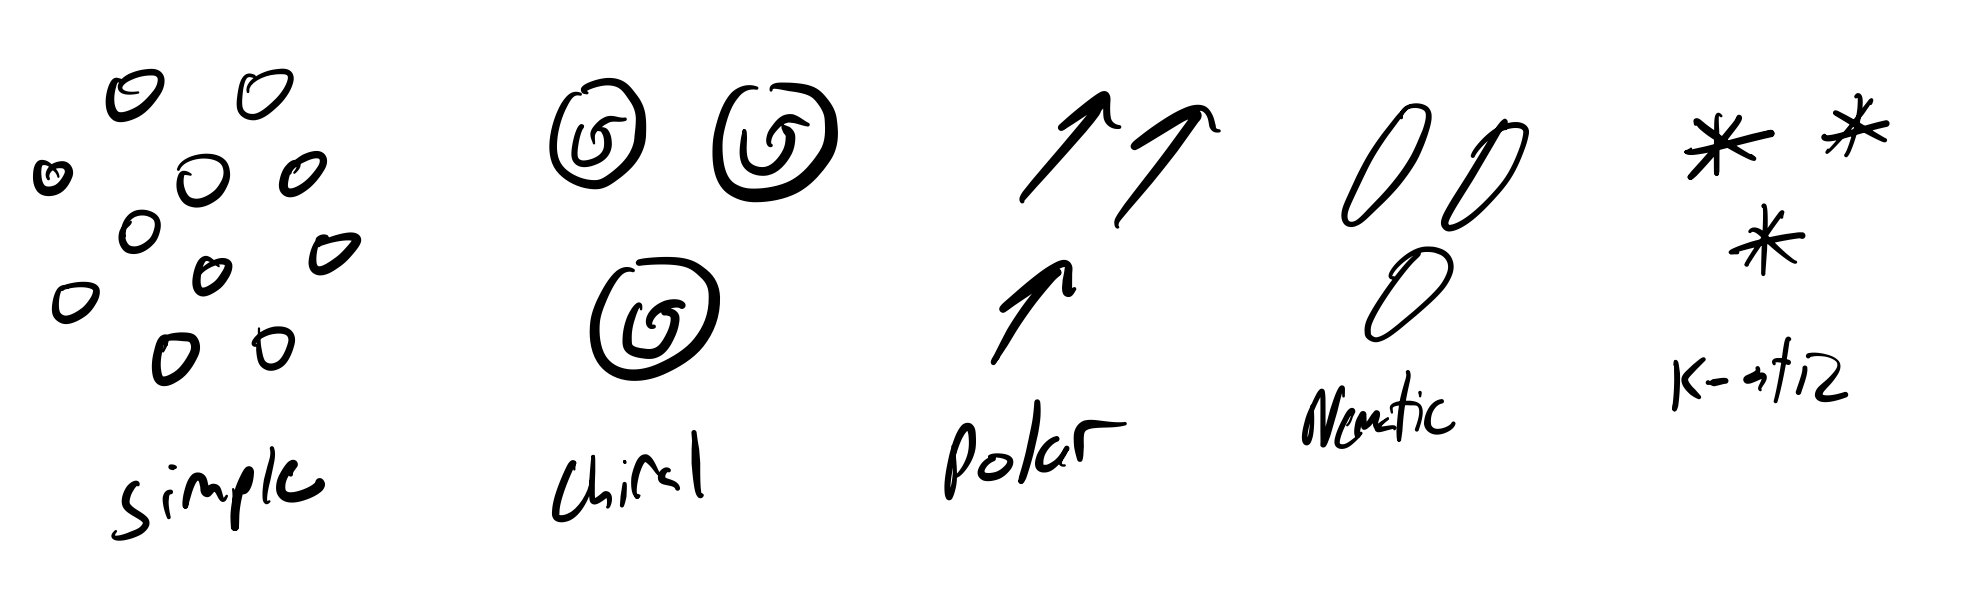
\includegraphics[scale=0.4]{Lectures/Images/lec17-particles.png}
\end{center}

\subsection{MIPS (qualitatively)}
Today we will study scalar active fluids - for such fluids, injecting energy at the microscopic scale for such fluids gives us motility-induced phase separation, or MIPS\footnote{A video of which can be found here \url{https://www.youtube.com/watch?v=H0kou04dylE}}. 

If we just have a box of gas, the probability that they may spontaneously form a water droplet is vanishingly small. In order to get such phase separation in a passive fluid, we need attraction in between molecules, so that the energy associated with them being together is greater than the entropy gain associated with them being farther apart. But interestingly, for active fluids we spontaneously have phase separation, with only repulsive interactions.

We need two ingredients for MIPS:
\begin{itemize}
    \item Repulsive interactions of some form.
    \item Self-propulsion. However, unlike the Viczek model we discussed a couple weeks ago, there is no preferred orientation of the fluid. Each individual particle has an individual polarity, but the fluid as a whole has a total polarity of zero.
\end{itemize}

Qualitatively, how can we see MIPS arise? 
\begin{enumerate}
    \item We first observe (tautologically) that particles spend more time in regions where they move slower.
    \item Particles move slower when their motility is cancelled out by a pairwise collision.
    \item Such particles make a bigger/better target in phase space for other particles to collide with; this target will be stationary. This causes more particles to accumulate. Note that after we form such a region, only particles as the boundaries of such regions have a chance of escaping.
\end{enumerate}

Let's see if we can see MIPS arise quantitatively. We start by reviewing Brownian motion.

\subsection{Brownian Motion and Langevin Dynamics}
We start with a review of classical equilibrium Brownian motion, and then add activity.

Scottish Botanist Robert Brown (1827) noticed pollen grains jiggled; he noticed that a repeated experiment with dead particles still jiggled, so such motion was not due to life. 

Then, many decades later, Albert Einstein (1905) used a course-grained description to derive some properties of Brownian motion:
\begin{equation}
    \frac{\overline{x^2}}{2t} = D = \frac{RT}{6\pi \eta r N_A}
\end{equation}

with $D$ the diffusion coefficient, $R$ the gas constant, $T$ the temperature, $\eta$ the viscosity, $r$ the radius of the spheres, $N_A$ Avogadro's constant. This made a connection between a particle diffusing via Brownian motion and atomic physics, allowing people to estimate the atomic length scale and the amount of atoms in a mole $N_A$.

Marian Smoluchowski gave an idealized argument for why Brownian particles stay in motion.

Finally (though there are many others that worked on this area) Paul Langevin bravely wrote down a (stochastic) differential equation for the motion of an individual diffusing particle. He was also a cool dude\footnote{He was an outspoken anti-fascist, was removed from his position under Nazi rule, but fortunately survived to see the liberation of Paris.}

Let's first think about our favourite dimensionless constant, the Reynolds number:
\begin{equation}
    \text{Re} = \frac{\rho u L}{\eta}
\end{equation}

\begin{center}
    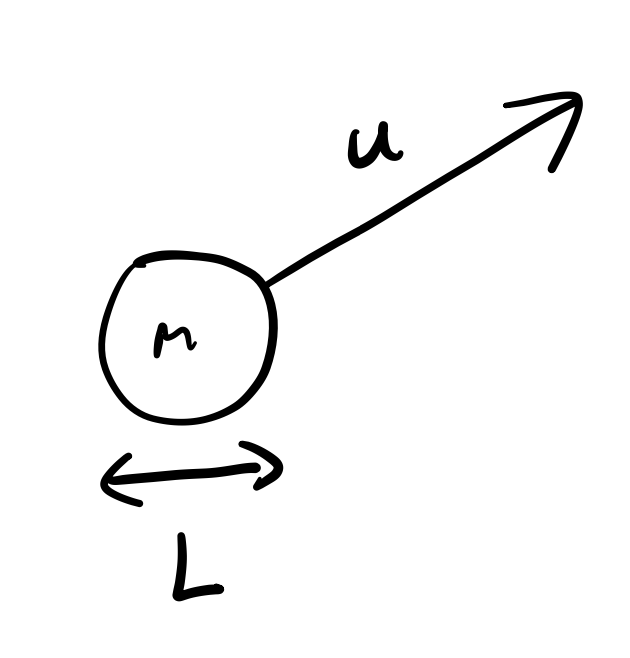
\includegraphics[scale=0.4]{Lectures/Images/lec17-colloid.png}
\end{center}

If we have $L \sim 10\mu\si{m}, m \sim 10\mu\si{m s^{-1}}, \eta/\rho \sim 10^{-6}\si{m^2s^{-1}}$, then the Reynolds number is $\text{Re} \sim 10^{-4} \ll 1$, so We can take the Navier Stokes equation:
\begin{equation}
    \rho D_t\v{v} = \eta \nabla^2 \v{v} - \nabla p + \v{F}_{\text{body}}(\v{r})
\end{equation}
and set the inertial term to zero (Stokes' regime)
\begin{equation}
    0 = \eta \nabla^2 \v{v} - \nabla p + \v{F}_{\text{body}}(\v{r})
\end{equation}
We can then use this to derive the drag force on a sphere moving through fluids using Green's function methods:
\begin{equation}
    F_{\text{drag}} = -6\pi \eta r U
\end{equation}

\begin{center}
    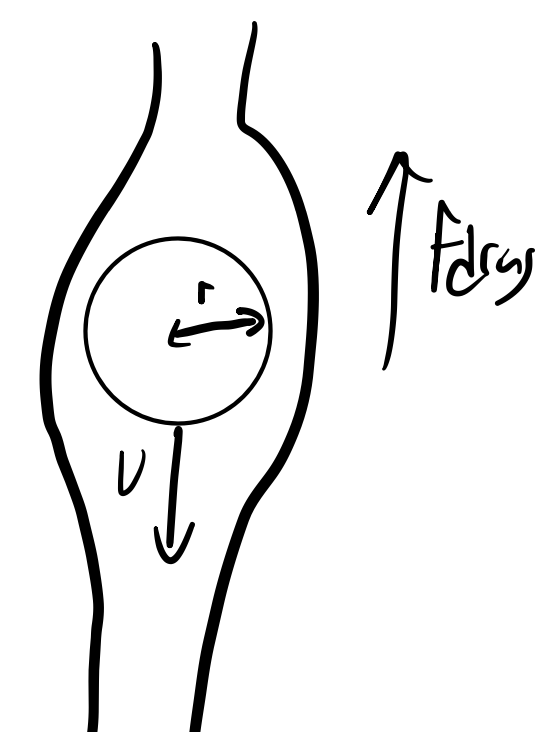
\includegraphics[scale=0.4]{Lectures/Images/lec17-stokesdrag.png}
\end{center}

The net force on the pollen grain is then (using Newton's second law):
\begin{equation}
    m\dod{U}{t} = F_{\text{drag}} + F_{\text{collisions}}
\end{equation}
Or defining $\Gamma = \frac{6\pi \eta r}{M}$:
\begin{equation}
    \boxed{\dod{U}{t} = -\Gamma U + L(t)}
\end{equation}
where $L(t) = F_{\text{collisions}}/m$, is a strongly, quickly fluctuating stochastic term. This is the Langevin equation. So we have a drag term corresponding to exponential decay, in addition to a stochastic term that is sampled every moment in time from an ensemble. Often, people assume that the noise term is drawn from a Gaussian distribution:
\begin{equation}
    \overline{L(t)} = 0
\end{equation}
\begin{equation}
    \overline{L(t)L(t')} = 2\gamma\delta(t-t')
\end{equation}
with $\gamma$ being the fluctuation strength. The $\delta$ correlations means that there is no memory, and the solution will hence be a Markov process - there will be no dependence on the current state of the system on past moments.

Again neglecting the inertial term/making a further approximation, we get the equation for Brownian dynamics:
\begin{equation}
    U(t) = \frac{1}{\Gamma}L(t)
\end{equation}

Note that $\gamma$ can be sometimes obtained from the microscopic physics, but oftentimes it is a phenomelogical paramter for us to figure out.

% The Langevin equations we have written down is pretty poorly defined if we think about it too hard (we need tools developed by Stratonovich and Ito)

\subsection{Course-Graining}
We want a process of going from individual microcopic trajectories to an ensemble/probability distribution:
\begin{equation}
    X(t) \to \set{X(t)} \to P(X, t)dX
\end{equation}
the result will be a Fokker-Planck equation:
\begin{equation}
    \dpd{P(X, t)}{t} = \ldots
\end{equation}
There is not a unique way to coarse grain a generic stochsastic system, because different people are interested in different things, and coarse graining involves making certain approximations/throwing away information. But for Langevin:
\begin{equation}
    \dod{X}{t} = a(X) + bL(t)
\end{equation}
we have that this exactly coarse grains into:
\begin{equation}
    \dpd{P(X, t)}{t} = -\dpd{[a(X)P]}{X} + \gamma\dpd[2]{[b^2P]}{X}
\end{equation}

More generally, coarse graining can be studied by the derivation of the Dean equation; namely, if we have:
\begin{equation}
    \frac{\text{d}\v{R}^{\alpha}}{\text{d}t} = \sum_{\beta=1}^{N}\v{F}(\v{R}^\alpha(t) - \v{R}^{\beta}(t)) + \v{G}(\v{R}^{\alpha}(t)) + \gv{\eta}^\alpha(t)
\end{equation}
Where:
\begin{equation}
    \xi^\alpha_i(t)\xi^\beta_j(t') = 2T\delta_{ij}\delta^{\alpha\beta}\delta(t-t')
\end{equation}
We have the density:
\begin{equation}
    \rho(\v{R}, t) = \sum_{\alpha=1}^N\delta(\v{R}^\alpha(t) - \v{R})
\end{equation}
And through a course graining procedure, we obtain the Dean equation:
\begin{equation}
    \dpd{\rho}{t} = T\nabla^2 \rho - \nabla \cdot \left[\v{G}(\v{R})\rho(\v{R}, t) + \int d^d \v{R}'\v{F}(\v{R} - \v{R}')\rho(\v{R}, t)\rho(\v{R}', t)\right] + \gv{\eta}(\v{R}, t)
\end{equation}
where $\gv{\eta}(\v{R}, t)$ is a stochastic field sastisfying
\begin{equation}
    \eta(\v{R}, t)\eta(\v{R}', t') = 2T \delta_{ij}\delta^{(d)}(\v{R} - \v{R}')\delta(t-t')
\end{equation}
As you have time, it is recommended to look at problems 3.10 (deriving Dean equation), 3.11 (deriving the Fokker-Planck equation from Dean), 9.2 (deriving the Toner-Tu equations from Dean). so you can see this machinery in detail. These are some of the most challenging problems in the book, but are worth doing!

We also introduce the master equation; this is the most general equation we could write to desribe the time evolution of a probability density. Labelling the states by $n$:
\begin{equation}
    \dot{P}_n(t) = \sum_{n'}W_{n'\to n}P_{n'}(t) - W_{n\neq n'}P_n(t)
\end{equation}
Where detailed balance is given by:
\begin{equation}
    W_{n'\to n}P^{\text{eq}}_n = W_{n\to n'}P^{\text{eq}}_{n'}
\end{equation}

For hopping on a 1D lattice:
\begin{equation}
    W_{n \to n'} = 0 \text{ unless } n' = n \pm 1 \quad \text{locality}
\end{equation}
\begin{equation}
    \begin{split}
        W_{n + 1 \to n} &= W_{n'+1 \to n'} = W_{\text{left}}
        \\ W_{n - 1 \to n} &= W_{n'-1 \to n'} = W_{\text{right}} \quad \text{(homogeneity)}
    \end{split}
\end{equation}
\begin{equation}
    W_{\text{left}} + W_{\text{right}} = 1 \quad \text{(unitarity)}
\end{equation}
Writing $W_{\text{right}} = \frac{1}{2} + \e, W_{\text{left}} = \frac{1}{2}-\e$, we get:
\begin{equation}
    \dot{P}_n = \left(\frac{1}{2} - \e\right)P_{n+1} + \left(\frac{1}{2} + \e\right)P_{n-1} - P_n = \frac{P_{n+1} - 2P_n + P_{n-1}}{2} - \e(P_{n+1} - P_{n-1}) = \frac{1}{2}\dpd[2]{P_n}{n} - \e\dpd{P_n}{n}
\end{equation}
Replacing $n = xa$ with $a$ the lattice spacing, then we arrive at the Fokker-Planck equation! This is in some sense the classical analog of the Schrodinger equation.

\subsection{MIPS (quantitatively)}
We consider two different models; the first is the active Brownian particle model:
\begin{equation}
    \dod{\v{r}_n}{t} = v_0\hat{\v{u}}(\theta_n) - \frac{1}{\gamma}\sum_{m\neq n}\nabla_n V(\v{r}_m - \v{r}_n)
\end{equation}
\begin{equation}
    \dod{\theta_n}{t} = \sqrt{2 D_\theta}\eta_n
\end{equation}
where:
\begin{equation}
    \overline{\eta_m(t)\eta_{n}(t')} = \delta_{mn}\delta(t-t')
\end{equation}

We also have the run-and-tumble model:
\begin{equation}
    \dod{\theta_n}{t} = \begin{cases}
        \sqrt{2D_\theta}\eta_n & \text{if } \abs{t - nT} < \e
        \\ 0 & \text{otherwise}
    \end{cases}
\end{equation}

The difference between the two models just being that either the noise is continuous or the particles run, and then stochastically rotate. ABPs well-describe colloids, while RTPs well-describe bacteria. Both give the same Fokker-Planck equation (the starting point ot your homework):
\begin{equation}
    \p_t P(\v{r}, \theta, t) = -\hat{\v{u}}(\theta)\cdot \nabla[\v{v}(\v{r})P(\v{r}, \theta, t)] + D_\theta\p_\theta^2P(\v{r}, t, \theta)
\end{equation}

and both give rise to MIPS dynamics. The ending point of your homework is as follows; you do a linear stability analysis on the fields, and find that the fluctuations of the fourier modes evolve as:
\begin{equation}
    \p_t \delta \rho(\v{q}, t) = -\frac{v(\rho_0)}{2D_\theta}[v(\rho_0) + \rho_0\left.\dpd{v}{\rho}\right|_{\rho_0}]q^2\delta \rho(\v{q}, t)
\end{equation}
The only thing that could be negative is the derivative term, and this gives the quantiative picture of MIPS based on stability based on whether this term changes sign. If you want to read more about this, check out chapter 8 on the spinoidal decomposition.

\subsection{References}
\begin{itemize}
    \item A minimum of stochastics for Scientists (Noel Corngold)
    \item Active Matter: from motility to self-organization, Boulder school on Self-organizing matter July 2024 (M. Cristina Marchetti) - check out part 3 for help with the homework.
\end{itemize}
